With a quantum circuit parametrized by $U(\kvec,\thv)$, VQAs employ a classical optimization algorithm in order to minimize the cost-function in Eq.~\eqref{eq:cost}. Here, we will focus on derivative-based methods, which at each cycle $\ell$ of the algorithm, the gradient $\nabla _{\thv} C(\kvec,\thv)$ is computed, and a cost-minimizing direction is followed. Ussually, the initial parameters $\thv^{\ell}$ are randomly chosen (this random initialization should be understood according to the Haar measure, as we discuss in the next Section). In the following we will first discuss about optimization algorithms, and then on how such gradients can be computed.

The most straightforward approach in gradient-based optimization is that of following the gradient; as such we are guaranteed to attain (at least) a local minima. Thus, in Gradient Descent algorithm, the continuous parameters are updated according to
\begin{equation}\label{eq:GD}
\thv^{(\ell + 1)} = \thv^{(\ell)} - \alpha \nabla _{\thv}(\kvec,\thv)|_{\thv = \thv^{(\ell)}},
\end{equation}
where $\alpha$ is the \textit{learning-rate}, accounting for the update-step size, and this is guaranteed to reach, at least, a local-minima.

In optimization problems where the dataset is too large, computing the gradients can be prohibitively expensive (for instance, if the entire dataset does not fit in the memory). In this case, the training set is splitted into chunks, and an stochasticity arises when estimating gradient; such is the case of Stochastic Gradient Descent (SGD), where the gradient is estimated out of $b$-dimensional data subsets known as \textit{batches}. At each cycle, the data is randomly splitted and the update rule of Eq.~\ref{eq:GD} is sequentially applied using the gradient $\nabla _{\thv} C(\kvec,\thv)$ computed using each batch (note that this injects stochasticity); an \textit{epoch} is consequently defined as an entire pass of the original training set. We note that this stochasticity, which might in principle appear undesired, it can actually be helpful since taking random directions often help in escaping local minima.

While a large learning-rate value in Eq.~\ref{eq:GD} can potentially forbid the optimizer to reach the actual minima (since the update becomes simply \textit{too large}), we note that small learning-rate values will potentially dampen the convergence rate. More elaborate optimization algorithms can be considered, which adapt the magnitude of the learning-rate according to the gradient landscape at hand. Among them, a very popular optimizer is the Adaptive Moment Estimation (Adam) algorithm~\cite{kingma2015adam}, which sequentially adapts the learning rate for each parameter, by specifically tailoring it out from moving averages of first and second moments for each gradient component. In practice, this allows to reach a better optimization performance, although we shall ultimately adapt the optimization algorithm to the specific problem at hand. In the context of VQA, many issues need to be addressed, such as shot-noise, sampling-complexity and optimal choice of learning-rate values to take into account the quantum nature of the optimization landscape; in this regard there has been a tremendous effort in developing quantum-aware optimizers~\cite{verdon2018universal,kubler2020adaptive,arrasmith2020operator,stokes2020quantum,koczor2019quantum,nakanishi2020sequential,fontana2020optimizing,gu2021adaptive}.

With a basic understanding on how optimization algorithms proceed, let us now discuss how the essential ingredient in the update-rule can be obtained under the VQA framework. For this, we distinguish between two approaches: \textit{(i)} classical simulation of quantum circuits, and \textit{(ii)} experimental implementations on quantum hardware.

\subsubsection{Classical simulation of quantum circuits $\&$ Automatic differentiation}
If no particular symmetries are imposed, we are able to simulate quantum systems classically for up to $\sim 30$ qubits\footnote{On the contrary, many systems can be approximated efficiently by using clever ansatzes; this lies at the heart of Tensor Network (TN) methods such as Matrix Product States (MPS), Density Matrix Renormalization Group (DMRG) or Multiscale Entanglement Renormalization Ansatz (MERA). There is currently much excitement about TNs: while the space of all possible quantum states is large, only a portion of it is \textit{physically relevant} and it is believed that such portion can be simulated efficiently using TNs~\cite{Biamonte2017tensornetworks,orusTN}.}.
%
State-of-the-art techniques used to classically compute VQA-cost-function gradients rely on automatic differentiation (AD), in which cost-function derivatives are obtained by tracking each intermmediate-operation derivative, and following the chain-rule~\cite{broughton2020tensorflow,Luo2020yaojlextensible}. This is done by decomposing a generic program in terms of elementary operations whose derivatives can be computed, and is the spirit behind the paradigm of \textit{differentiable programming}~\cite{Rackauckas2020GeneralizedPL,Liao2019differentaible,dpcontrolsto}.

We remark that AD differs from numerical differentiation (such as finite differences) since it is an exact method. Similarly to symbolic differentiation, each operation involved in the computation provides a rule for its derivative with respect to the corresponding input. However, the output of AD is a numerical value of the derivative, and not a mathematical expression for it.

In turn, AD is carried out by constructing a \textit{computational graph}, where nodes are associated to the elementary operations present in the computation (and whose derivatives are known), and where the dependence on the parameters is explicited. In order to compute the function derivative, the graph is transversed either forward or backwards; the latter case is known as \textit{backpropagation}\footnote{The optimal way to transverse the computational graph generally depends on the setting at hand. For high-dimensional inputs (as customary when working with neural networks), backpropagation is prefered at the cost of an increase in memory usage.}. Thanks to efficient matrix multiplication sub-routines and special-purpose hardware such as GPUs and TPUs, this can be done consideraly fast, and in turn AD stands as one of the main ideas behind the advent of Artificial Intelligence.

\begin{figure}[t!]
    \centering
    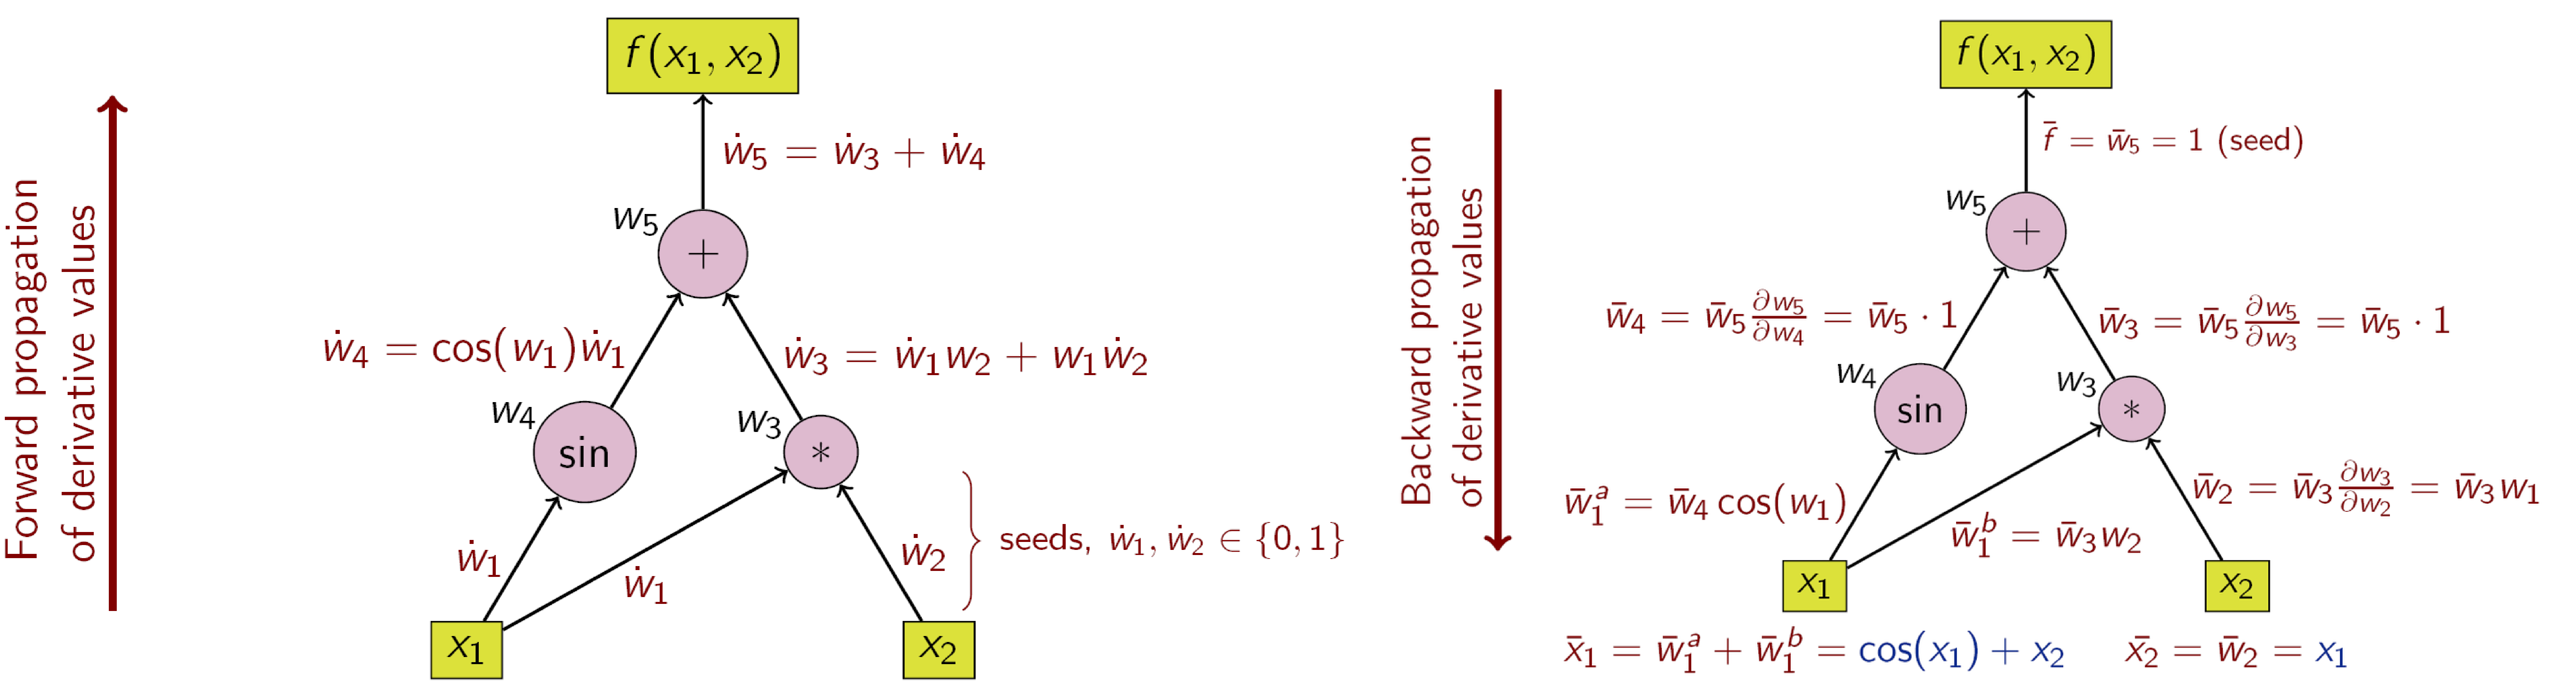
\includegraphics[width=1.\textwidth]{Figures/ad.pdf}
    \caption{We show how the computational graph is travelled forward and backwards in each of the possible modes of AD, for the example of an scalar function $f(x_1,x_2) = x_1 x_2 + \sin(x_1)$}
    \label{fig:ad}
\end{figure}

Let us consider an example\footnote{Taken from Ref.~\cite{wikiAD}} of an algorithm taking as input a real-value $x$, and outputing $y = f(g(h(x))$ where $f,g$ and $h$ are elementary functions whose derivatives are well-known and can be recorded when building the computational graph. We aim to compute $\partial_x y$, and to this end we define $w_0 = x$, $w_1 = h(w_0)$, $w_2 = g(w_1)$ and $w_3 = f(w_2) = y$. Now, the chain rule implies that
\equ{\frac{\partial y}{\partial x} = \frac{\partial y}{\partial w2} \frac{\partial w2}{\partial w1}  \frac{\partial w1}{\partial x}.} Thus, the computational graph is built by recording each of the elementary functions that need to be computed \textit{and} each of the elementary functions derivatives, which are known in advance. Then, forward-AD transverses the chain-rule from inside to outside, by first computing $\frac{\partial w_1}{\partial x}$, then $\frac{\partial w_2}{\partial w_1}$ and finally $\frac{\partial y}{\partial w_2}$.
On the contrary, backwards-AD transverses the chain-rule from outside to inside, by first computing $\frac{\partial y}{\partial w_2}$, then $\frac{w_2}{w_1}$ and finally $\frac{\partial w_1}{\partial x}$. As a concrete example, we can consider the function
\begin{align}
y &= f(x_1, x_2) \\
&= x_1 x_2 + \sin(x_1) \\ 
&= w_1 w_2 + \sin(w_1) \\
&= w_3 + w_4 \\
&= w_5,
\end{align}
where at each elementary operation we define a new variable $w_i$, which represents a node in the computational-graph. In the table we show the operations needed to compute the function, forward-AD, and backward-AD (this is also schematised in Fig.~\ref{fig:ad}).
\begin{center}
\begin{tabular}{| c |c |c |}
\hline
Function computation  &  Forward-AD&  Backward-AD\\
\hline
  $w_1 = x_1$&  $\dot{w}_1 = 1$ (\texttt{seed})&  $\bar{w}_5 = 1$ \texttt{seed}\\
  \hline
  $w_2 = x_2 $&  $\dot{w}_1 = 0$ (\texttt{seed})&  $\bar{w}_4 = \bar{w}_5 \cdot 1$\\
  \hline
  $w_3 = w_1\cdot w_2$& $\dot{w}_3 = \dot{w}_1\cdot w_2+ w_1 \cdot \dot{w}_2$ &  $\bar{w}_3 = \bar{w}_5 \cdot 1$\\
  \hline
  $w_4 = \sin(w_1)$& $\dot{w}_4 = \cos(w_1)\cdot \dot{w}_1$  &  $\bar{w}_2 = \bar{w}_3 \cdot w_1$\\
  \hline
  $w_5 = w_3 + w_4$& $\dot{w}_5 = \dot{w}_3 + \dot{w}_4$ &  $\bar{w}_1 = \bar{w}_3 \cdot w_2 + \bar{w}_4 \cos(w_1)$\\
  \hline
\end{tabular}
\end{center}
Here, we used the notation of $\bar{w}_i=\frac{\partial y}{\partial w_i}$ for the backward-AD, and note that the \textit{seed value} in this example is trivial for such case (since it stands for possible multidimensional outputs, \textit{e.g.} cases where $y \in \mathbb{R}^n$). On the contrary, since the example function has two inputs $(x_1, x_2)$, forward-AD needs to be specified which derivative we are computing ---either $\partial_{x_1} y$, as set by the seed value in the table, or $\partial_{x_2} y$---. Note that to compute the gradient, we would need two passes of the graph for this example\footnote{For a vector field $f:\mathbb{R}^m\rightarrow \mathbb{R}^n$, then computing the gradient requires $m$
computational graphs sweeps for the backward-AD, and $n$ sweeps for the forward-AD.}.

While this discussion only provides an introduction to the meaning of AD, we remark that much work has been done in this field during the last years, and we refer the interested reader to Refs.~\cite{wikiAD,abadi2016tensorflow,maclaurinautograd,maclaurin2016phd,survey_ad}.

\subsubsection{Experimental implementations on quantum hardware}
In NISQ circuits, backpropagating cost-function derivatives imply that the quantum state at each step in the circuit should be kept in memory, a fact essentially forbiden because of exponentially large Hilbert-spaces. Alternatively, we can use quantum hardware to compute such gradients.

In this scenario, cost-function derivatives can be obtained by the so-called \textit{parameter-shift rules} where cost-function derivatives are expressed as linear combinations of cost-function values, each obtained by using the very same circuit, but shifting the parameters by a finite amount. We remark that this is an analytic result, unrelated to numerical differentiation techniques such as finite differences\footnote{In turn, finite-differences do not get along with gradient-based optimizers, and often leads to inestabilities due to approximation errors; this issue intensifies in the NISQ framework, since we generally need to resolve between cost-function values that are small. Estimating such difference in cost-function values turns difficult, since not only a high amount of samples is required, but also the strong presence of hardware-noise can potentially forbid to resolve it.}.

In the following we will detail the idea behind parameter-shift rules. Let us consider a single parameter $\alpha \in \thv$, and a VQE problem, whose Hamiltonian is $\hat{H}$ and thus the cost-function becomes %(see also Eq.~\ref{eq:vqe_cost})
\begin{equation}
C(\thv) = C_{\text{VQE}}(\thv)= \expect{0|U^\dagger(\thv) \hat{H}U(\thv)|0},
\end{equation}
where we momentaneaously simplified our notation by dropping the dependence on $\kvec$, and used the notation $\ket{0}^{\otimes n} \equiv \ket{0}$).

Moreover, we will assume that $U(\thv) = U_L G(\alpha) U_R$, where $U_L$ and $U_R$ are unitary transformations parametrized by $\thv - \llaves{\alpha}$. Upon defining $\ket{\psi} = U_R \ket{0}$, and $\hat{Q} = U_L^\dagger \hat{H}U_L$, it follows that
\begin{align}\label{eq:shifted}
\partial_\alpha C(\thv) =& \expect{\psi |G^\dagger \hat{Q} (\partial_\alpha G)| \psi} + \expect{\psi |(\partial_\alpha G^\dagger) \hat{Q} \partial_\alpha G| \psi},\end{align}
where we used $G$ as a shorthand for $G(\alpha)$. Now, let us consider $G(\alpha) = e^{-\ii \frac{\alpha}{2} P}$, %$ = \cos(\frac{\alpha}{2}) - \ii \sin(\alpha) P$,
with $P \in \llaves{\sigma_x, \sigma_y, \sigma_z}$. In this case, we obtain
\begin{align}
\partial_\alpha C(\thv) =& \frac{\ii}{2}\expect{\psi |G^\dagger \Comm{P}{\hat{Q}} G |\psi}.\end{align}
Now, using the following identity, which holds for any operator $\sigma$~\cite{shiftrules1}:
\equ{\Comm{P}{\sigma} = \ii \Big( G(\frac{\pi}{2}) \sigma G(-\frac{\pi}{2}) - G(-\frac{\pi}{2}) \sigma G(\frac{\pi}{2}) )\Big),}
we get
\begin{align*}
\partial_\alpha C(\thv) =& -\frac{1}{2}\Big(\expect{\psi |G(\alpha)^\dagger G^\dagger(-\frac{\pi}{2}) \hat{Q} G(-\frac{\pi}{2}) G(\alpha)|  \psi}  + \expect{\psi |G(\alpha)^\dagger G^\dagger(\frac{\pi}{2}) \hat{Q} G(\frac{\pi}{2}) G(\alpha)|  \psi} \Big)
\end{align*}
By noting that $G(\alpha)G(\beta) = G(\alpha + \beta)$, and recalling that $\hat{Q} = U_L^\dagger \hat{H}U_L$, it follows that
\begin{equation}\label{eq:der}
\partial_\alpha C(\thv) = \frac{1}{2}\big(C(\thv)|_{\alpha \leftarrow \alpha + \frac{\pi}{2}} - C(\thv)|_{\alpha \leftarrow \alpha - \frac{\pi}{2}}\big)
\end{equation}
This procedure can be extended to consider arbitrary Pauli strings~\cite{shiftrules1}, and unitary transformations for which the derivative is not unitary. In the latter case, the derivative can be written as a linear combination of unitary operations, resulting in a generalized parameter-shift rule which --- as opposed to Eq~\ref{eq:der} --- involves more than two contributions~\cite{shiftrules2, Wierichs2022generalparameter}.

Thus, the cost-function derivatives can be obtained by estimating each term in Eq.~\ref{eq:der} using a quantum computer parametrized by $U(\thv)$, and repeating this procedure for each parameter $\alpha \in \thv$. As mentioned, this result is exact (contrary to numerical differentiation methods); it nevertheless relies on cost-function estimates, thus statistical fluctuations arising from measurement outcomes will always be present. This plays an important role if the value of such derivatives is small, in which case many measurements will be required in order to deal with sufficient accuracy.

Thus, VQAs' optimizers will generally need to deal with an intrinsically stochastic component, and convergence properties of SGD has been analyzed in Ref.~\cite{Sweke2020}. Following such reference, we can readily distinguish between different sources of \textit{stochasticity}, the first one being shot-noise. Alternatively, in Eq.~\ref{eq:decoH} we have decomposed the Hamiltonian as a sum of Pauli-string, and at each cycle of the optimization algorithm, the gradient could be estimated out of a subset of all the Pauli strings present in such decomposition. In this case, another source of stochasticity arises, and is associated to estimating cost-function gradient out of a subset of terms appearing in the cost-function. Methods combining both techniques are known as \textit{doubly-stochastic} optimizers~\cite{Sweke2020,harrow2019low}.

Overall, parameter-shift rules can be understood as a \textit{recipe} for computing gradients of cost functions; we remark that the approach presented above naturally generalizes to cost-functions of the form in Eq.~\ref{eq:cost}. Under this recipe, circuit's structure needs not to be modified, but rather the parameter in question is shifted, and the derivative is obtained as linear combination of the corresponding cost-function estimates. For classical simulation purposes, the \textit{best of both worlds} are ussually combined, and backpropagation methods are used along with the parameter-shift rules (provided that the systems under consideration are not too large); this is one among the many efforts behind projects like TensorFlow-Quantum or PennyLane ~\cite{bergholm2018pennylane,broughton2020tensorflow}.

By now, we have introduced the basic ingredients required to run a VQA. Namely, a strategy that defines the structure of our quantum circuit, a cost-function that evaluates its performance, and a (classical) optimization algorithm that takes control of free parameters such as rotation values. The ultimate goal is to find the global minima of the cost function by navigating the optimization landscape. In this regard many issues have been recently raised up, which put into question the overall feasibility of VQA framework, and that is the matter of our next section.
